\documentclass{article}

\usepackage{arxiv}

\usepackage[utf8]{inputenc} % allow utf-8 input
\usepackage[T1]{fontenc}    % use 8-bit T1 fonts
\usepackage{lmodern}        % https://github.com/rstudio/rticles/issues/343
\usepackage{hyperref}       % hyperlinks
\usepackage{url}            % simple URL typesetting
\usepackage{booktabs}       % professional-quality tables
\usepackage{amsfonts}       % blackboard math symbols
\usepackage{nicefrac}       % compact symbols for 1/2, etc.
\usepackage{microtype}      % microtypography
\usepackage{lipsum}
\usepackage{graphicx}

\title{Vaccinating Australia: How long will it take?}

\author{
    Mark Hanly
   \\
    Centre for Big Data Research in Health \\
    UNSW Sydney \\
  Sydney 2052 \\
  \texttt{\href{mailto:m.hanly@unsw.edu.au}{\nolinkurl{m.hanly@unsw.edu.au}}} \\
   \And
    Tim Churches
   \\
    Ingham Institute for Applied Medical Research \\
    South Western Sydney Clinical School, Faculty of Medicine, UNSW Sydney \\
  Liverpool \\
  \texttt{\href{mailto:timothy.churches@unsw.edu.au}{\nolinkurl{timothy.churches@unsw.edu.au}}} \\
   \And
    Oisín Fitzgerald
   \\
    Centre for Big Data Research in Health \\
    UNSW Sydney \\
  Sydney 2052 \\
  \texttt{\href{mailto:o.fitzgerald@unsw.edu.au}{\nolinkurl{o.fitzgerald@unsw.edu.au}}} \\
   \And
    C Raina McIntyre
   \\
    Biosecurity Research Program, The Kirby Institute \\
    UNSW Sydney \\
  Sydney 2052 \\
  \texttt{\href{mailto:rainam@protonmail.com}{\nolinkurl{rainam@protonmail.com}}} \\
   \And
    Louisa Jorm
   \\
    Centre for Big Data Research in Health \\
    UNSW Sydney \\
  Sydney 2052 \\
  \texttt{\href{mailto:l.jorm@unsw.edu.au}{\nolinkurl{l.jorm@unsw.edu.au}}} \\
  }


% Pandoc citation processing

\usepackage{booktabs}
\usepackage{longtable}
\usepackage{array}
\usepackage{multirow}
\usepackage{wrapfig}
\usepackage{float}
\usepackage{colortbl}
\usepackage{pdflscape}
\usepackage{tabu}
\usepackage{threeparttable}
\usepackage{threeparttablex}
\usepackage[normalem]{ulem}
\usepackage{makecell}
\usepackage{xcolor}


\begin{document}
\maketitle

\def\tightlist{}


\begin{abstract}
Add abstract here.
\end{abstract}

\keywords{
    COVID19
   \and
    vaccination
  }

\newpage

\hypertarget{introduction}{%
\section{Introduction}\label{introduction}}

The development and regulatory approval of multiple safe and efficacious
COVID-19 vaccines in less than a year is a truly remarkable achievement.
The logistical task of administering the vaccine rapidly and fairly to
billions of people around the world will be no less of a challenge.
National vaccination programs have commenced in many countries including
Israel, the United States and the United Kingdom. Here in Australia, the
government has entered into four agreements for the supply of COVID-19
vaccines (Table \ref{tab:agreements}), with a view to starting
distribution in late February, and an ambitious target to finish
vaccinating the adult community in October.\textsuperscript{1} This
gives around 35 weeks to administer two doses each to some 20 million
adult Australians.

\begin{table}[H]

\begin{threeparttable}
\caption{\label{tab:agreements}Australia’s vaccine agreements}
\centering
\begin{tabular}[t]{>{\raggedright\arraybackslash}p{3cm}>{\raggedright\arraybackslash}p{3cm}>{\centering\arraybackslash}p{2cm}>{\raggedright\arraybackslash}p{2cm}>{\raggedright\arraybackslash}p{4cm}}
\toprule
Name & Type & Doses (millions) & Schedule & Status\\
\midrule
\cellcolor{gray!6}{Pfizer/BioNTech} & \cellcolor{gray!6}{mRNA vaccine} & \cellcolor{gray!6}{10} & \cellcolor{gray!6}{2 doses 21 days apart} & \cellcolor{gray!6}{Provisionally approved by the TGA}\\
University of Oxford AstraZeneca & Viral vector vaccine & 54 & 2 doses 28 days apart & Phase 3 clinical trials\\
\cellcolor{gray!6}{Novavax} & \cellcolor{gray!6}{Protein vaccine} & \cellcolor{gray!6}{51} & \cellcolor{gray!6}{2 doses 21 days apart} & \cellcolor{gray!6}{Phase 3 clinical trials}\\
COVAX Facility & Assorted & 25 & Assorted & 9 candidate vaccines in various clinical trial stages\\
\bottomrule
\end{tabular}
\begin{tablenotes}
\small
\item [] Adapted from https://www.health.gov.au/initiatives-and-programs/covid-19-vaccines/about-covid-19-vaccines/australias-vaccine-agreements
\end{tablenotes}
\end{threeparttable}
\end{table}

The national roll-out strategy divides the population into 16 groups,
organised into five distinct phases (Table \ref{tab:phases}). Hospital
hubs with access to cold chain storage facilities will administer the
Pfizer/BioNTech vaccine to the highest priority groups scheduled in
Phase 1a, which includes border workers, frontline healthcare staff, and
aged care staff and residents. Pending approval, the Astra Zeneca
vaccine would be administered to the bulk of the population through a
network of GPs and pharmacies. The Prime Minister Scott Morrison has
quoted a target of 80,000 vaccinations per day,\textsuperscript{2}
however a back of the envelope calculation would suggest that at this
rate it would take some 500 days to vaccinate 20 million adult
Australians twice, placing the finish line somewhere around the middle
of 2022. To reach the October target would take closer to 160,000 daily
vaccinations.

When it comes to vaccine roll-out, speed is of the essence. Statistical
modelling has illustrated that epidemic duration, cases and deaths are
minimised dramatically as the number of available daily vaccinations
increases. For example, increasing the daily capacity by 25\% from
75,000 to 100,000 would see a 60\% reduction in total cases and
deaths.\textsuperscript{3}

An added complication is that the Pfizer/BioNTech and AstraZeneca
vaccines both require two doses---a primer and a booster---which need to
be delivered within a specified time frame after the initial shot. This
complicates roll-out as the daily resources of both vaccine units and
healthcare staff must be divided between those waiting for their first
jab and those returning for their booster.

\begin{table}[H]

\begin{threeparttable}
\caption{\label{tab:phases}Australia’s COVID-19 vaccine national roll-out strategy}
\centering
\begin{tabular}[t]{>{\raggedright\arraybackslash}p{1cm}>{\raggedright\arraybackslash}p{11cm}>{\raggedleft\arraybackslash}p{2cm}}
\toprule
Phase & Description & Size\\
\midrule
\textbf{\cellcolor{gray!6}{1a}} & \cellcolor{gray!6}{Quarantine \& border workers} & \cellcolor{gray!6}{70,000}\\
\textbf{1a} & Frontline health care workers & 100,000\\
\textbf{\cellcolor{gray!6}{1a}} & \cellcolor{gray!6}{Aged care and disability care staff} & \cellcolor{gray!6}{318,000}\\
\textbf{1a} & Aged care and disability care residents & 190,000\\
\textbf{\cellcolor{gray!6}{1b}} & \cellcolor{gray!6}{Elderly adults aged 80 years and over} & \cellcolor{gray!6}{1,045,000}\\
\textbf{1b} & Elderly adults aged 70-79 years & 1,858,000\\
\textbf{\cellcolor{gray!6}{1b}} & \cellcolor{gray!6}{Other health care workers} & \cellcolor{gray!6}{953,000}\\
\textbf{1b} & Aboriginal and Torres Strait Islander people aged 55 years and over & 87,000\\
\textbf{\cellcolor{gray!6}{1b}} & \cellcolor{gray!6}{Younger adults with an underlying medical condition} & \cellcolor{gray!6}{2,000,000}\\
\textbf{1b} & Critical and high risk workers & 196,000\\
\textbf{\cellcolor{gray!6}{2a}} & \cellcolor{gray!6}{Adults aged 60-69} & \cellcolor{gray!6}{2,650,000}\\
\textbf{2a} & Adults aged 50-59 & 3,080,000\\
\textbf{\cellcolor{gray!6}{2a}} & \cellcolor{gray!6}{Aboriginal and Torres Strait Islander people aged 18-54} & \cellcolor{gray!6}{387,000}\\
\textbf{2a} & Other critical and high risk workers & 453,000\\
\textbf{\cellcolor{gray!6}{2b}} & \cellcolor{gray!6}{Balance of adult population} & \cellcolor{gray!6}{6,643,000}\\
\textbf{3} & <18 if recommended & 5,670,000\\
\bottomrule
\end{tabular}
\begin{tablenotes}
\small
\item [] Adapted from https://www.health.gov.au/sites/default/files/documents/2021/01/australia-s-covid-19-vaccine-national-roll-out-strategy.pdf
\end{tablenotes}
\end{threeparttable}
\end{table}

Another unknown is the question of vaccine hesitancy, which refers to
the delay in acceptance or refusal to take a vaccine despite one being
available.\textsuperscript{4} Clearly, high levels of vaccine hesitancy
would have the potential to undermine efforts to vaccinate the
population. An online survey of over 3,000 Australian adults undertaken
in August 2020 asked respondents if they would take a safe and effective
vaccine for COVID-19, if one was developed. The population-weighted
responses were 5.5\% ``definitely not'', 7.2\% ``probably not'', 28.7\%
``probably'' and 58.5\% ``definitely''.\textsuperscript{5} This suggests
relatively low levels of vaccine hesitancy, however this could still be
problematic. At the time of writing it seems likely that the bulk of the
Australian population will receive the Astra Zeneca vaccine, which has
recorded an average efficacy of 70\% across clinical trial
arms.\textsuperscript{6} At this level, it would be necessary to
immunise 86\% of the entire population to achieve herd
immunity.\textsuperscript{3}

The aim of this analysis is to estimate how long it will take to
distribute the two-dose COVID-19 vaccine schedule to the Australian
population. We consider a variety of scenarios based on the daily
vaccine capacity, the time frame between the first and second dose and
the scale of vaccine hesitancy in the population. We conclude by
comparing daily vaccination rates from countries where vaccination
programs are already underway.

\hypertarget{methods}{%
\section{Methods}\label{methods}}

\hypertarget{population-and-priority-groups}{%
\subsection{Population and priority
groups}\label{population-and-priority-groups}}

Our analysis was based on the 16 priority groups and five phases
proposed by the Australian government (see Table \ref{tab:phases}). Th
implied population size is 25.7 million people, including 5.67 million
children and adolescents under the age of 18. We assumed that equal
priority was given to all groups within the same phase.

\hypertarget{vaccine-roll-out-projections}{%
\subsection{Vaccine roll out
projections}\label{vaccine-roll-out-projections}}

Roll out projections were based on four parameters:

\begin{enumerate}
\def\labelenumi{\arabic{enumi}.}
\tightlist
\item
  The daily vaccination capacity.
\item
  The minimum number of days between the first dose and the second dose.
\item
  The maximum number of days between the first dose and the second dose.
\item
  Vaccine hesitancy
\end{enumerate}

\hypertarget{projection-scenarios}{%
\subsection{Projection scenarios}\label{projection-scenarios}}

Projection scenarios were based on a \(2^k\) factorial design defined by
three factors with two levels each. The scenarios are summarised in
Table \ref{tab:scenarios} and the three factors and levels are detailed
below:

\begin{itemize}
\item
  Daily vaccination capacity (80,000 versus 170,000)
\item
  Timing between first and second dose (3-6 weeks versus 3-12 weeks)
\item
  Vaccine hesitancy (7\% versus 13\%).
\end{itemize}

\begin{table}[H]

\caption{\label{tab:scenarios}Projection scenarios}
\centering
\begin{tabu} to \linewidth {>{}l>{\raggedleft}X>{\raggedleft}X>{\raggedleft}X}
\toprule
Scenario & Capacity (units per day) & Gap between doses & Hesitancy\\
\midrule
\textbf{\cellcolor{gray!6}{1}} & \cellcolor{gray!6}{80,000} & \cellcolor{gray!6}{3 to 6 weeks} & \cellcolor{gray!6}{7\%}\\
\textbf{2} & 80,000 & 3 to 6 weeks & 13\%\\
\textbf{\cellcolor{gray!6}{3}} & \cellcolor{gray!6}{80,000} & \cellcolor{gray!6}{3 to 12 weeks} & \cellcolor{gray!6}{7\%}\\
\textbf{4} & 80,000 & 3 to 12 weeks & 13\%\\
\textbf{\cellcolor{gray!6}{5}} & \cellcolor{gray!6}{170,000} & \cellcolor{gray!6}{3 to 6 weeks} & \cellcolor{gray!6}{7\%}\\
\textbf{6} & 170,000 & 3 to 6 weeks & 13\%\\
\textbf{\cellcolor{gray!6}{7}} & \cellcolor{gray!6}{170,000} & \cellcolor{gray!6}{3 to 12 weeks} & \cellcolor{gray!6}{7\%}\\
\textbf{8} & 170,000 & 3 to 12 weeks & 13\%\\
\bottomrule
\end{tabu}
\end{table}

The projections assumed that those who were hesitant would never receive
the vaccine. The range of hesitancy rates were based on the survey data
reported by Edwards et al,\textsuperscript{5} and only applied to
general population groups. Border staff, healthcare and aged care
workers, aged care residents and adults with a medical condition were
assumed to have 0\% vaccine hesitancy.

\hypertarget{vaccine-allocation}{%
\subsection{Vaccine allocation}\label{vaccine-allocation}}

We allocated the daily available vaccination doses according to the
following algorithm:

\begin{enumerate}
\def\labelenumi{\arabic{enumi}.}
\item
  Calculate the number of second doses due, based on the specified
  permissible range for the second dose. As an example, if the second
  dose is is specified to be administered between 3 and 6 weeks, then
  the booster shots for people vaccinated on day 1 would be evenly
  distributed across the three weeks between day 22 and day 42).
\item
  Assign the remaining doses from the daily limit to those awaiting
  their first dose.
\item
  Identify the highest priority phase that haven't received all first
  doses.
\item
  Divide the available first doses between the subgroups in the highest
  priority phase, proportional to the number of unvaccinated individuals
  remaining in each subgroup.
\item
  Stop when all population members, minus those who are hesitant, have
  been vaccinated twice.
\end{enumerate}

\hypertarget{software-and-code}{%
\subsection{Software and code}\label{software-and-code}}

The analysis was performed using R version 4.0.3. The source code can be
accessed at \url{https://github.com/CBDRH/vaccinatingAustralia}.

\hypertarget{results}{%
\section{Results}\label{results}}

Results from the eight scenarios are presented in Table
\ref{tab:scenarios}. Scenarios that assumed a vaccine hesitancy of 7\%
among the general population resulted in 48.3 million vaccine doses
administered to 24.2 million people, corresponding to a population
coverage of 94.0\%. Scenarios that assumed the vaccine higher hesitancy
rate of 13\% resulted in 45.7 million vaccine doses administered to 22.9
million people for a coverage of 88.9\%.

Under an most optimistic Scenario of 200,000 daily doses with the 7\%
hesitancy rate (Scenario 5), assuming a start date of 1 March, Phase 1a
would be fully vaccinated (i.e.~primer and booster doses administered)
as early as 13 April---just six weeks. The entire adult population would
be fully vaccinated by 25 October---in line with government
targets---and a further eight weeks would see the entire population
include those under 18 vaccinated. Under this optimistic scenario, the
vulnerable groups in Phase 2a, including adults aged 70 and above and
those with underlying medical conditions, would be fully vaccinated
before the onset of the colder winter months. Under this scenario, we
would reach 50\% population coverage in late July and 75\% population
Around the start of October (Figure \ref{fig:cumlResults}A).

\begin{table}[H]

\caption{\label{tab:projections}Summary of vaccine roll-out projections for different scenarios}
\centering
\begin{tabu} to \linewidth {>{}l>{\raggedleft}X>{\raggedleft}X>{\raggedleft}X>{\raggedright}X>{\raggedleft}X>{\raggedleft}X>{\raggedleft}X>{\raggedright}X}
\toprule
Scenario & Number of vaccinations (millions) & Individuals vaccinated (millions) & Population coverage (\%) & Phase 1a complete & Phase 1b complete & Phase 2a complete & Phase 2b complete & Phase 3 complete\\
\midrule
\textbf{\cellcolor{gray!6}{1}} & \cellcolor{gray!6}{48.3} & \cellcolor{gray!6}{24.2} & \cellcolor{gray!6}{94.0} & \cellcolor{gray!6}{18/04/21} & \cellcolor{gray!6}{04/09/21} & \cellcolor{gray!6}{08/02/22} & \cellcolor{gray!6}{11/07/22} & \cellcolor{gray!6}{20/11/22}\\
\textbf{2} & 45.7 & 22.9 & 88.9 & 18/04/21 & 01/09/21 & 22/01/22 & 18/06/22 & 19/10/22\\
\textbf{\cellcolor{gray!6}{3}} & \cellcolor{gray!6}{48.3} & \cellcolor{gray!6}{24.2} & \cellcolor{gray!6}{94.0} & \cellcolor{gray!6}{30/05/21} & \cellcolor{gray!6}{09/10/21} & \cellcolor{gray!6}{10/03/22} & \cellcolor{gray!6}{13/08/22} & \cellcolor{gray!6}{23/12/22}\\
\textbf{4} & 45.7 & 22.9 & 88.9 & 30/05/21 & 05/10/21 & 23/02/22 & 19/07/22 & 20/11/22\\
\textbf{\cellcolor{gray!6}{5}} & \cellcolor{gray!6}{48.3} & \cellcolor{gray!6}{24.2} & \cellcolor{gray!6}{94.0} & \cellcolor{gray!6}{13/04/21} & \cellcolor{gray!6}{15/06/21} & \cellcolor{gray!6}{19/08/21} & \cellcolor{gray!6}{25/10/21} & \cellcolor{gray!6}{22/12/21}\\
\textbf{6} & 45.7 & 22.9 & 88.9 & 13/04/21 & 05/06/21 & 20/07/21 & 17/09/21 & 07/11/21\\
\textbf{\cellcolor{gray!6}{7}} & \cellcolor{gray!6}{48.3} & \cellcolor{gray!6}{24.2} & \cellcolor{gray!6}{94.0} & \cellcolor{gray!6}{25/05/21} & \cellcolor{gray!6}{26/06/21} & \cellcolor{gray!6}{07/09/21} & \cellcolor{gray!6}{30/10/21} & \cellcolor{gray!6}{27/12/21}\\
\textbf{8} & 45.7 & 22.9 & 88.9 & 25/05/21 & 25/06/21 & 01/09/21 & 21/10/21 & 13/12/21\\
\bottomrule
\end{tabu}
\end{table}

Under the less optimistic scenarios of 80,000 doses administered daily,
it would take until June to August 2022 to vaccinate the adult
population (Table \ref{tab:scenarios}). Under Scenario 1, we would reach
50\% population coverage in January 2022 and 75\% population coverage in
July 2022 (Figure \ref{fig:cumlResults}B).

\begin{figure}

{\centering 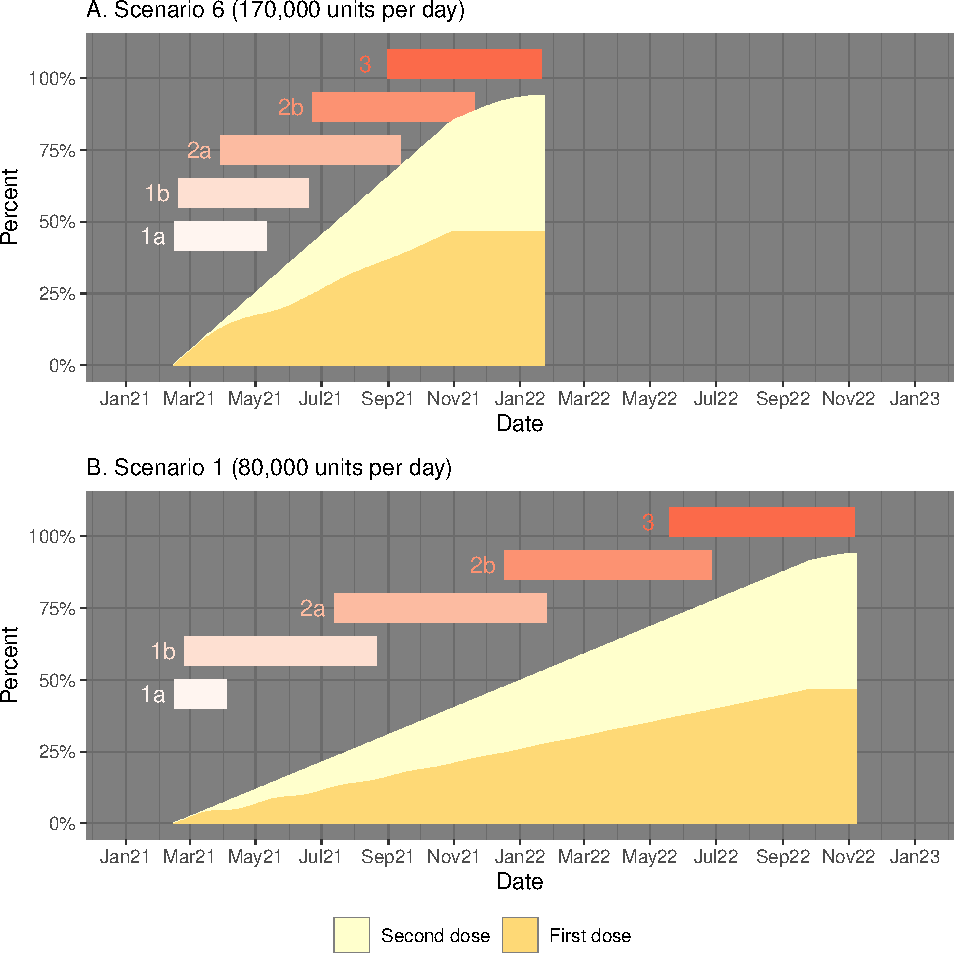
\includegraphics{researchNote_files/figure-latex/cumlResults-1} 

}

\caption{Cumulative vaccine doses over time}\label{fig:cumlResults}
\end{figure}

\hypertarget{discussion}{%
\section{Discussion}\label{discussion}}

To meet the target of vaccinating all amenable adult Australians by the
end of October 2021 there will need to be in the order of 200,000 doses
delivered daily on average---a truly furious pace.

To put bounds on the feasibility of this target, a potentially
illuminating exercise is to compare to the vaccination rates achieved by
other countries who have already begun to roll out their vaccination
programs (Figure \ref{fig:dailyVac}. The stand out leader is Israel,
where between 7,000 and 20,000 vaccinations per million population have
been delivered daily through out January. Several factors have
contributed to this success, including a young, centralised population
and a strong public health infrastructure. Perhaps most important has
been strong logistical planning, including coordination of delivery,
cold-chain storage and staffing.\textsuperscript{7} Other countries have
been less successful in their roll-out, including the United States
(4,000 per million pop), the United Kingdom (5,000 per million pop) and
the European Union (1,100 per million pop).

With a population of 25.7 million in Australia, the figure of 200,000
doses per day from our projections corresponds to around 7,800 daily
doses per million population. It will be possible to vaccinate the
Australian population in just eight months but we will need to do
considerably better than the rates currently being achieved in most
countries. Completing vaccination roll-out this year is possible, but it
will require dedicated large-scale vaccination sites that are capable of
delivering thousands of doses a day as well as the enthusiastic
participation of GP practices and community pharmacies around the
country. We need to start now, get up to speed quickly and maintain that
pace. The recent invitation extended to community pharmacies to
participate in the vaccination roll-out is a welcome development. There
are some 5,800 community pharmacies across Australia; if each could
vaccinate 20 community members a day that would represent half of the
target of 200,000 daily doses to cross the finish line for community
vaccination by the end of October.

\begin{verbatim}
## $caption
## [1] "Data source: ourworldindata.org"
## 
## attr(,"class")
## [1] "labels"
\end{verbatim}

\begin{figure}

{\centering 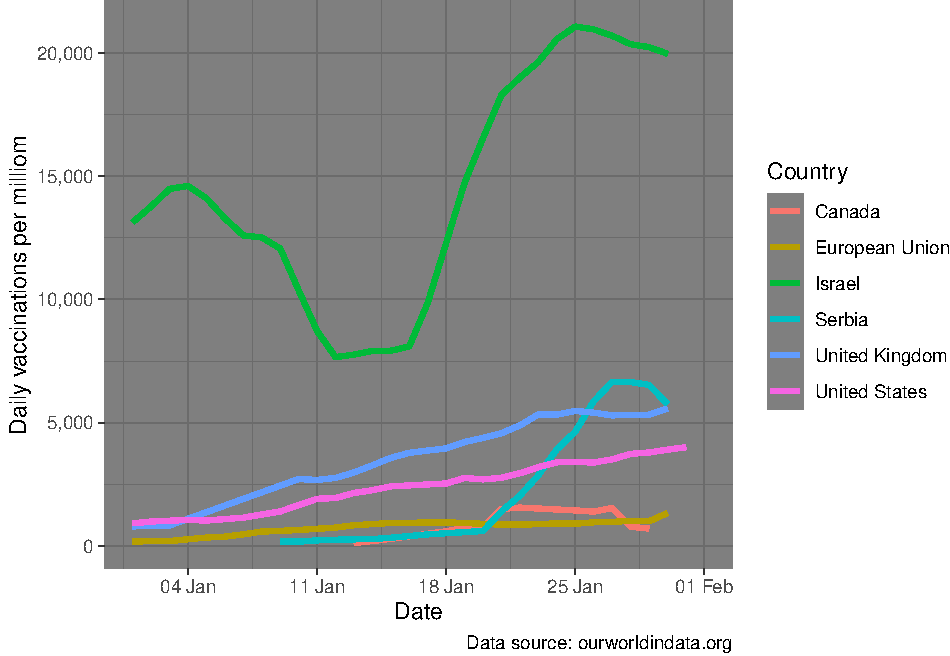
\includegraphics{researchNote_files/figure-latex/dailyVac-1} 

}

\caption{Daily COVID-19 vaccines administered per one million population}\label{fig:dailyVac}
\end{figure}

\newpage

\hypertarget{references}{%
\section*{References}\label{references}}
\addcontentsline{toc}{section}{References}

\hypertarget{refs}{}
\leavevmode\hypertarget{ref-gh2021a}{}%
1. Health AGD of. Doorstop interview on 31 january 2021.
\emph{Australian Government Department of Health}. Published online
January 2021.
\url{https://www.health.gov.au/ministers/the-hon-greg-hunt-mp/media/doorstop-interview-on-31-january-2021}

\leavevmode\hypertarget{ref-pm2021}{}%
2. Press conference - australian parliament house. Published online
January 2021.
\url{https://www.pm.gov.au/media/press-conference-australian-parliament-house-12}

\leavevmode\hypertarget{ref-macintyre2020modelling}{}%
3. MacIntyre CR, Costantino V, Trent MJ. Modelling of covid-19
vaccination strategies and herd immunity, in scenarios of limited and
full vaccine supply in nsw, australia. \emph{medRxiv}. Published online
2020.

\leavevmode\hypertarget{ref-macdonald2015vaccine}{}%
4. MacDonald NE, others. Vaccine hesitancy: Definition, scope and
determinants. \emph{Vaccine}. 2015;33(34):4161-4164.

\leavevmode\hypertarget{ref-edwards2020covid}{}%
5. Edwards B, Biddle N, Gray M, Sollis K. COVID-19 vaccine hesitancy and
resistance: Correlates in a nationally representative longitudinal
survey of the australian population. \emph{medRxiv}. Published online
2020.

\leavevmode\hypertarget{ref-voysey2020safety}{}%
6. Voysey M, Clemens SAC, Madhi SA, et al. Safety and efficacy of the
chadox1 nCoV-19 vaccine (azd1222) against sars-cov-2: An interim
analysis of four randomised controlled trials in brazil, south africa,
and the uk. \emph{The Lancet}. 2020;397(10269):99-111.

\leavevmode\hypertarget{ref-mckee2021can}{}%
7. McKee M, Rajan S. What can we learn from israel's rapid roll out of
covid 19 vaccination? \emph{Israel Journal of Health Policy Research}.
2021;10(1):1-4.

\bibliographystyle{unsrt}
\bibliography{references.bib}


\end{document}
